\documentclass{standalone}
\usepackage{tikz}
\usetikzlibrary{patterns, positioning}

\begin{document}
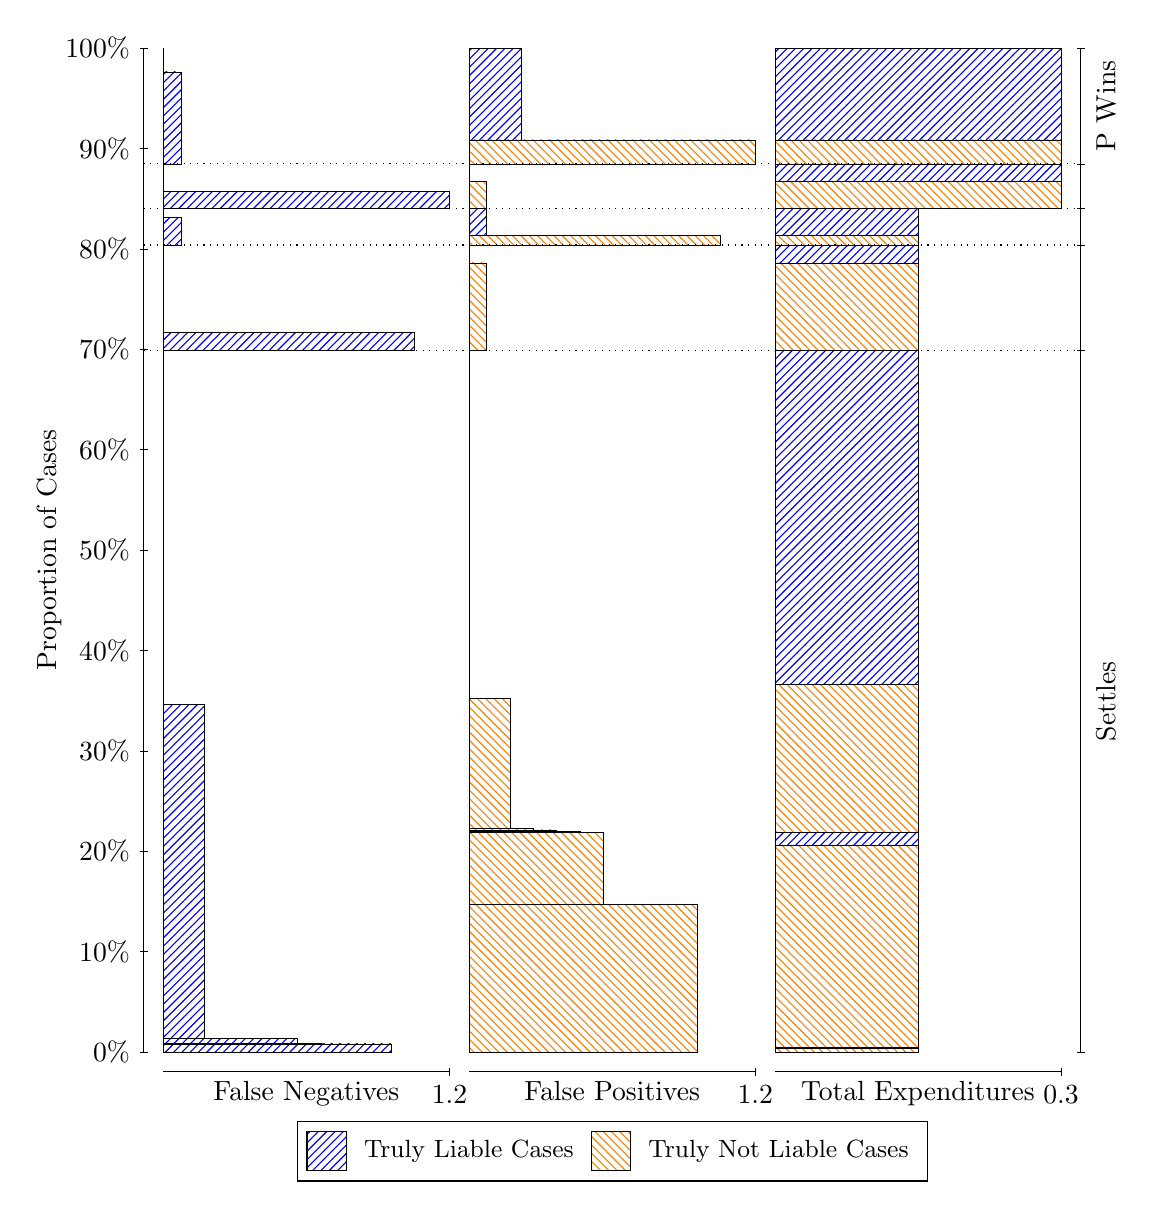
\begin{tikzpicture}
\draw[black, very thin] (1.5,1.75) -- (1.5,14.5);
\node[rotate=90, anchor=center] at (0.3, 8.125) {Proportion of Cases};
\draw[black, very thin] (1.45,1.75) -- (1.55,1.75);
\node[anchor=east] at (1.45, 1.75) {0\%};
\draw[black, very thin] (1.45,3.025) -- (1.55,3.025);
\node[anchor=east] at (1.45, 3.025) {10\%};
\draw[black, very thin] (1.45,4.3) -- (1.55,4.3);
\node[anchor=east] at (1.45, 4.3) {20\%};
\draw[black, very thin] (1.45,5.575) -- (1.55,5.575);
\node[anchor=east] at (1.45, 5.575) {30\%};
\draw[black, very thin] (1.45,6.85) -- (1.55,6.85);
\node[anchor=east] at (1.45, 6.85) {40\%};
\draw[black, very thin] (1.45,8.125) -- (1.55,8.125);
\node[anchor=east] at (1.45, 8.125) {50\%};
\draw[black, very thin] (1.45,9.4) -- (1.55,9.4);
\node[anchor=east] at (1.45, 9.4) {60\%};
\draw[black, very thin] (1.45,10.675) -- (1.55,10.675);
\node[anchor=east] at (1.45, 10.675) {70\%};
\draw[black, very thin] (1.45,11.95) -- (1.55,11.95);
\node[anchor=east] at (1.45, 11.95) {80\%};
\draw[black, very thin] (1.45,13.225) -- (1.55,13.225);
\node[anchor=east] at (1.45, 13.225) {90\%};
\draw[black, very thin] (1.45,14.5) -- (1.55,14.5);
\node[anchor=east] at (1.45, 14.5) {100\%};

\draw[black, very thin] (13.4,1.75) -- (13.4,14.5);
\draw[black, very thin] (13.35,1.75) -- (13.45,1.75);
\node[anchor=west] at (13.35, 1.75) {};
\draw[black, very thin] (13.35,10.659) -- (13.45,10.659);
\node[anchor=west] at (13.35, 10.659) {};
\draw[black, very thin] (13.35,11.998) -- (13.45,11.998);
\node[anchor=west] at (13.35, 11.998) {};
\draw[black, very thin] (13.35,12.463) -- (13.45,12.463);
\node[anchor=west] at (13.35, 12.463) {};
\draw[black, very thin] (13.35,13.03) -- (13.45,13.03);
\node[anchor=west] at (13.35, 13.03) {};
\draw[black, very thin] (13.35,14.5) -- (13.45,14.5);
\node[anchor=west] at (13.35, 14.5) {};

\draw[black, very thin, pattern color=blue, pattern=north east lines] (1.75,1.75) rectangle (4.6418,1.8514);
\draw[black, very thin, pattern color=blue, pattern=north east lines] (1.75,1.8514) rectangle (4.3452,1.8526);
\draw[black, very thin, pattern color=blue, pattern=north east lines] (1.75,1.8526) rectangle (4.0486,1.8539);
\draw[black, very thin, pattern color=blue, pattern=north east lines] (1.75,1.8539) rectangle (3.752,1.8553);
\draw[black, very thin, pattern color=blue, pattern=north east lines] (1.75,1.8553) rectangle (3.4554,1.9219);
\draw[black, very thin, pattern color=blue, pattern=north east lines] (1.75,1.9219) rectangle (3.1588,1.9222);
\draw[black, very thin, pattern color=blue, pattern=north east lines] (1.75,1.9222) rectangle (2.8622,1.9225);
\draw[black, very thin, pattern color=blue, pattern=north east lines] (1.75,1.9225) rectangle (2.5656,1.9228);
\draw[black, very thin, pattern color=blue, pattern=north east lines] (1.75,1.9228) rectangle (2.269,6.1652);
\draw[black, very thin, pattern color=orange, pattern=north west lines] (1.75,6.1652) rectangle (1.75,10.659);
\draw[black, very thin, pattern color=blue, pattern=north east lines] (1.75,10.659) rectangle (4.9384,10.886);
\draw[black, very thin, pattern color=orange, pattern=north west lines] (1.75,10.886) rectangle (1.75,11.998);
\draw[black, very thin, pattern color=blue, pattern=north east lines] (1.75,11.998) rectangle (1.9724,12.345);
\draw[black, very thin, pattern color=orange, pattern=north west lines] (1.75,12.345) rectangle (1.75,12.463);
\draw[black, very thin, pattern color=blue, pattern=north east lines] (1.75,12.463) rectangle (5.3833,12.684);
\draw[black, very thin, pattern color=orange, pattern=north west lines] (1.75,12.684) rectangle (1.75,13.03);
\draw[black, very thin, pattern color=blue, pattern=north east lines] (1.75,13.03) rectangle (1.9724,14.196);
\draw[black, very thin, pattern color=orange, pattern=north west lines] (1.75,14.196) rectangle (1.75,14.5);
\draw[black, very thin, pattern color=orange, pattern=north west lines] (5.6333,1.75) rectangle (8.5252,3.6223);
\draw[black, very thin, pattern color=orange, pattern=north west lines] (5.6333,3.6223) rectangle (8.2286,3.6235);
\draw[black, very thin, pattern color=orange, pattern=north west lines] (5.6333,3.6235) rectangle (7.932,3.6247);
\draw[black, very thin, pattern color=orange, pattern=north west lines] (5.6333,3.6247) rectangle (7.6354,3.6258);
\draw[black, very thin, pattern color=orange, pattern=north west lines] (5.6333,3.6258) rectangle (7.3388,4.5356);
\draw[black, very thin, pattern color=orange, pattern=north west lines] (5.6333,4.5356) rectangle (7.0422,4.5356);
\draw[black, very thin, pattern color=orange, pattern=north west lines] (5.6333,4.5356) rectangle (7.0422,4.5535);
\draw[black, very thin, pattern color=orange, pattern=north west lines] (5.6333,4.5535) rectangle (6.7456,4.5705);
\draw[black, very thin, pattern color=orange, pattern=north west lines] (5.6333,4.5705) rectangle (6.449,4.5868);
\draw[black, very thin, pattern color=orange, pattern=north west lines] (5.6333,4.5868) rectangle (6.1524,6.2436);
\draw[black, very thin, pattern color=blue, pattern=north east lines] (5.6333,6.2436) rectangle (5.6333,10.659);
\draw[black, very thin, pattern color=orange, pattern=north west lines] (5.6333,10.659) rectangle (5.8558,11.771);
\draw[black, very thin, pattern color=blue, pattern=north east lines] (5.6333,11.771) rectangle (5.6333,11.998);
\draw[black, very thin, pattern color=orange, pattern=north west lines] (5.6333,11.998) rectangle (8.8218,12.117);
\draw[black, very thin, pattern color=blue, pattern=north east lines] (5.6333,12.117) rectangle (5.8558,12.463);
\draw[black, very thin, pattern color=orange, pattern=north west lines] (5.6333,12.463) rectangle (5.8558,12.81);
\draw[black, very thin, pattern color=blue, pattern=north east lines] (5.6333,12.81) rectangle (5.6333,13.03);
\draw[black, very thin, pattern color=orange, pattern=north west lines] (5.6333,13.03) rectangle (9.2667,13.334);
\draw[black, very thin, pattern color=blue, pattern=north east lines] (5.6333,13.334) rectangle (6.3007,14.5);
\draw[black, very thin, pattern color=orange, pattern=north west lines] (9.5167,1.75) rectangle (11.333,1.8013);
\draw[black, very thin, pattern color=blue, pattern=north east lines] (9.5167,1.8013) rectangle (11.333,1.8052);
\draw[black, very thin, pattern color=orange, pattern=north west lines] (9.5167,1.8052) rectangle (11.333,4.3717);
\draw[black, very thin, pattern color=blue, pattern=north east lines] (9.5167,4.3717) rectangle (11.333,4.5397);
\draw[black, very thin, pattern color=orange, pattern=north west lines] (9.5167,4.5397) rectangle (11.333,6.4155);
\draw[black, very thin, pattern color=blue, pattern=north east lines] (9.5167,6.4155) rectangle (11.333,10.659);
\draw[black, very thin, pattern color=orange, pattern=north west lines] (9.5167,10.659) rectangle (11.333,11.771);
\draw[black, very thin, pattern color=blue, pattern=north east lines] (9.5167,11.771) rectangle (11.333,11.998);
\draw[black, very thin, pattern color=orange, pattern=north west lines] (9.5167,11.998) rectangle (11.333,12.117);
\draw[black, very thin, pattern color=blue, pattern=north east lines] (9.5167,12.117) rectangle (11.333,12.463);
\draw[black, very thin, pattern color=orange, pattern=north west lines] (9.5167,12.463) rectangle (13.15,12.81);
\draw[black, very thin, pattern color=blue, pattern=north east lines] (9.5167,12.81) rectangle (13.15,13.03);
\draw[black, very thin, pattern color=orange, pattern=north west lines] (9.5167,13.03) rectangle (13.15,13.334);
\draw[black, very thin, pattern color=blue, pattern=north east lines] (9.5167,13.334) rectangle (13.15,14.5);
\draw[black, dotted] (1.5,10.659) -- (13.4,10.659);
\draw[black, dotted] (1.5,11.998) -- (13.4,11.998);
\draw[black, dotted] (1.5,12.463) -- (13.4,12.463);
\draw[black, dotted] (1.5,13.03) -- (13.4,13.03);
\draw[black, very thin] (1.75,1.5) -- (5.3833,1.5);
\node[anchor=north] at (3.5667, 1.5) {False Negatives};
\draw[black, very thin] (5.3833,1.45) -- (5.3833,1.55);
\node[anchor=north] at (5.3833, 1.45) {1.2};

\draw[black, very thin] (5.6333,1.5) -- (9.2667,1.5);
\node[anchor=north] at (7.45, 1.5) {False Positives};
\draw[black, very thin] (9.2667,1.45) -- (9.2667,1.55);
\node[anchor=north] at (9.2667, 1.45) {1.2};

\draw[black, very thin] (9.5167,1.5) -- (13.15,1.5);
\node[anchor=north] at (11.333, 1.5) {Total Expenditures};
\draw[black, very thin] (13.15,1.45) -- (13.15,1.55);
\node[anchor=north] at (13.15, 1.45) {0.3};

\node[black, centered, rotate=90] at (13.72, 6.2044) {Settles};



\node[black, centered, rotate=90] at (13.72, 13.765) {P Wins};

\draw (7.449999999999999,1.5) node[draw=none] (baseCoordinate) {};
\begin{scope}[align=center]
        \matrix[scale=0.5, draw=black, below=0.5cm of baseCoordinate, nodes={draw}, column sep=0.1cm]{
            \node[rectangle, draw, minimum width=0.5cm, minimum height=0.5cm, pattern=north east lines, pattern color=blue] {}; &
            \node[draw=none, font=\small] (B) {Truly Liable Cases}; &
            \node[rectangle, draw, minimum width=0.5cm, minimum height=0.5cm, pattern=north west lines, pattern color=orange] {}; &
            \node[draw=none, font=\small] (B) {Truly Not Liable Cases}; \\
            };
\end{scope}

\end{tikzpicture}
\end{document}